\documentclass[a4paper]{article}

\usepackage{fullpage} % Package to use full page
\usepackage{parskip} % Package to tweak paragraph skipping
\usepackage{tikz} % Package for drawing
\usepackage{amsmath}
\usepackage{hyperref}

\title{MTH 4300: Algorithms, Computers, and Programming II}
\author{Fall 2024}
\date{Midterm Review}

\begin{document}
\maketitle


\section{TRUE OR FALSE}
\begin{enumerate}
    \item The command to compile and renamea file is: g++ main.cpp -o main
    \item Dockers MAIN purpose is to make programs faster
    \item the float data type takes up more memory in a program than the double
    \item while loops are used when you need a program to loop, 
          and the number of times it will loop is detetmined at run time.
    \item Is this syntax correct: int matrix[3][3] = \{1, 2, 3\},\{4, 5, 6\},\{7, 8, 9\};
    \item Base case for recursion is always required
    \item Arrays are technicaly pointers
    \item new is used to mark an item as never seen before
    \item A method refers to a private variable in a class
    \item All variables on the heap must be referenced using pointers
\end{enumerate}
\newpage


\section{SHORT ANSWER}
\begin{enumerate}
    \item Name one function defined inside iostream
    \item What is the terminal command to create a new folder?
    \item Fix the function below: \\
          void my\_function(int param1, param2)\\
          \{\\
          \text{    }cout$<$"hello"$<<$endl;\\
          \text{    }return 7;\\
          \}\\
    \item What is 28\%8 equal to?
    \item What does the sizeof function return ?
    \item Whats a disadvantage of recursion?
    \item Set a pointer to point to nothing
    \item Whats a dangling pointer and how is it caused.
    \item For private attributes of a class, what is the name of the special method used
          to set the values of the attributes?
    \item The variable int* pointer = \&x; is stored on the heap or the stack?
\end{enumerate}
\newpage 


\section{CODING}
\begin{enumerate}
    \item Write a c++ class to describe a toaster. Make sure to include at least
          3 attributes(set to private), 3 methods(set to public), and a 
          constructor(set to public). Write a main function and create 2 objects in the main. Figure out a way to print one 
          of your attributes in the main by calling one of your methods.
    \item Write a main function that creates a 5 by 5, 2d integer array(on the heap or 
          stack whatever you prefer). Then prompt the user to enter a row number x, and a value y. 
          For row x, fill up each entry with (y + column number).
    \item What does the following code print:\\\\
    \text{    }int x = 10;\\
    \text{    }int* y = \&x;\\
    \text{    }x=17;\\
    \text{    }*y=22;\\
    \text{    }cout$<<$x$<<$endl;\\
    \item What does the following code print:\\
    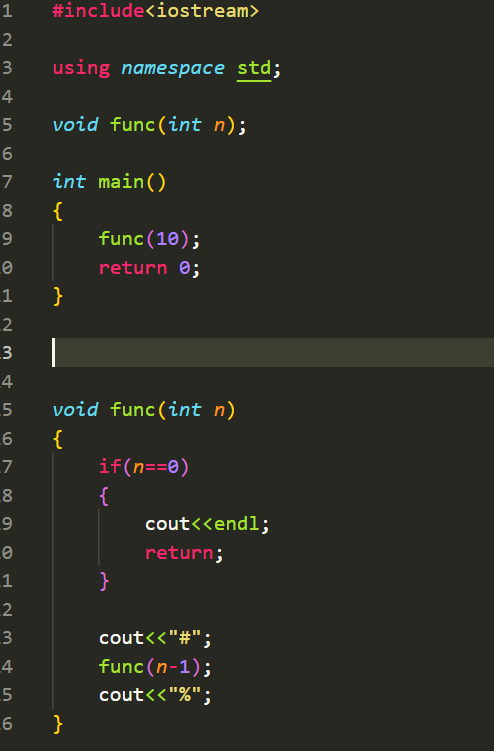
\includegraphics[width=5cm]{question2.png}
    
\end{enumerate} 
\newpage

\section{SOLUTIONS}
\subsection{TRUE OR FALSE}
\begin{enumerate}
    \item true
    \item false
    \item false
    \item true
    \item false
    \item true
    \item true
    \item false
    \item false
    \item true
\end{enumerate}

\subsection{SHORT ANSWER}
\begin{enumerate}
    \item cin
    \item mkdir
    \item int my\_function(int param1,int param2)\\
    {\\
    cout$<<$"hello"$<<$endl;\\
    return 7;\\
    }\\
    \item 4
    \item the number of bytes for the type of the input variable
    \item It can cause a stack overflow
    \item int* ptr=nullptr;
    \item When a pointer points to memory that has been freed. It is caused after
          you use the delete operator and forget to set the ptr to nullptr.
    \item constructor
    \item stack
\end{enumerate}

\subsection{CODING(files below located inside this repo)}
\begin{enumerate}
    \item \href{run:./coding_question1.cpp}{coding\_question1.cpp}
    \item \href{run:./coding_question2.cpp}{coding\_question2.cpp}
    \item \href{run:./coding_question3.cpp}{coding\_question3.cpp}
    \item \href{run:./coding_question4.cpp}{coding\_question4.cpp}
\end{enumerate}

\end{document}